\subsection{Restructuring}
After transitioning from cold geometry to hot geometry and evaluating the thermal expansion we have to take in account the fuel restructuring process.
We make some assumption about columnar and equiaxed region-radii, as well as on densities in different regions. We set the temperature boundaries for columnar ragion at 1800°C and at 1600°C for equiaxed region, according to Holander’s book. Regarding the densities, we consider that in the As-fabricated region the density remains the same, while in the equiaxed a percentage of TD of 95% and for the columnar a 98%. 
First of all, we evaluate columnar and equiaxed radii respectively at 1800°C and 1600°C as we said, based on a temperature map. This map provides the temperature at different heights along the fuel pin, using a precise function that allows us to determine the temperature at any position in the 3D model previously developed
Once  columnar and equiaxed radii are determined, we have to evaluate the void radius. The As-fabricated region is only the remaining potion of the fuel outer radius after subtracting the equiaxed region. Using this simple correlation to make a possible solution of void formation: 
\begin{equation}
R_{void} = \sqrt{
    R_{\text{col}}^2 - R_{\text{eq}}^2 \cdot \left( \frac{\text{Density}_{\text{AS}}}{\text{Density}_{\text{col}}} \right)
    + \left( R_{\text{eq}}^2 - R_{\text{col}}^2 \right) \cdot \left( \frac{\text{Density}_{\text{eq}}}{\text{Density}_{\text{AS}}} \right)
}
\end{equation}

At end, there is the plot of the fuel element: height vs Radius. We want to show the restructuring phenomenon and highlight the contributions’ dependence on the axial position-z of the fuel pin
Figure \ref{fig:restructuring} shows 

\begin{figure}[H]
\centering
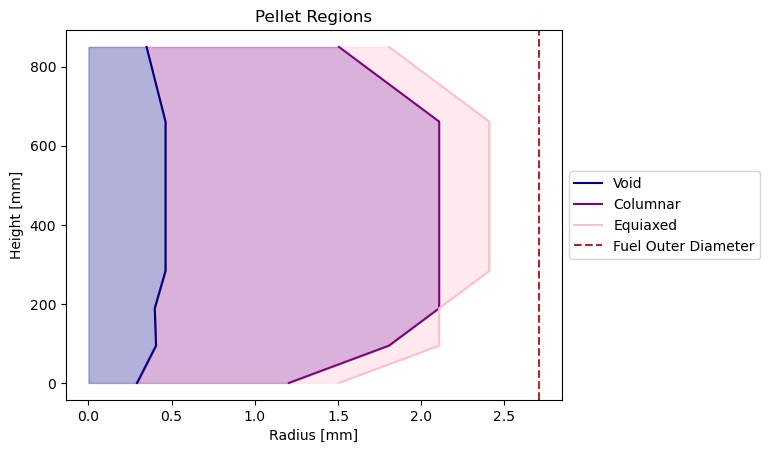
\includegraphics[width=0.8\textwidth]{restructuring.png}
\caption{Cladding swelling due to void formation.}
\label{fig:restructuring}
\end{figure}
